\documentclass[center,10pt,cm]{beamer}

\usepackage{listings}
% ----------
%  Packages
% ----------
\usepackage[latin1]{inputenc}
\usepackage[T1]{fontenc}
\usepackage{amsmath}
\usepackage{amsfonts}
\usepackage{amssymb}
\usepackage{fancyhdr}
\usepackage{float}
\usepackage{graphicx}

% -------------------------------
%  Optional packages (uncomment)
% -------------------------------
\usepackage{tikz}
%\usepackage{onimage}
%\usepackage{multirow}
%\usepackage{verbatim}
\usepackage{pstricks,pst-grad}
%\usepackage{hyperref} % links
%\usepackage{cancel}  % tachado en diagonal
%\usepackage{wasysym} % caritas
%\usepackage[normalem]{ulem} % tachado -> \sout{}
\usetikzlibrary{arrows,shapes,shadows,positioning}

\graphicspath{{./images/}} % Images folder

% --------------
%  Style config
% --------------
\usetheme{Boadilla}
\renewcommand{\arraystretch}{1.5}

\setbeamersize{text margin left=.2cm}
\setbeamersize{text margin right=.2cm}

\definecolor{mcolor}{HTML}{6187bb} % azulado
\definecolor{scolor}{HTML}{5ACE60} % green
\definecolor{mgray}{HTML}{4D4D4D}  % gray
\definecolor{sgray}{HTML}{9E9E9E}
\definecolor{tgray}{HTML}{E3E3E3}
\definecolor{agray}{HTML}{1C1C1C}

\definecolor{backgroundcolor}{gray}{0.96}
\definecolor{keywordcolor}{HTML}{2592EA}
\definecolor{commentcolor}{HTML}{EA252F}
\definecolor{stringcolor}{HTML}{D4C95E} %EAE025}

\setbeamercolor*{frametitle}{bg=mcolor,fg=white}
%%\setbeamercolor*{frametitle}{bg=white,fg=mcolor}
\setbeamercolor*{item}{fg=agray}
\setbeamercolor*{title}{fg=mcolor}
\setbeamercolor*{author}{fg=mgray}
\setbeamercolor*{institute}{fg=mgray}
\setbeamercolor*{date}{fg=mgray}
\setbeamercolor*{structure}{fg=mcolor}
\setbeamercolor*{footline}{fg=white, bg=mgray}

\renewcommand\mathfamilydefault{\rmdefault}
\renewcommand\familydefault{\rmdefault}
\setbeamerfont{title}{family*={fouriernc}, size=\fontsize{30}{32}}
\setbeamerfont{author}{family*={fouriernc}, size=\large}
\setbeamerfont{block body}{size*={8}{0}, family*={fouriernc}}
\setbeamerfont{block title}{size*={8}{0}, family*={fouriernc}}

%% \setbeamertemplate{itemize item}{\tiny\raise.2ex\hbox{\donotcoloroutermaths$\bullet$}}
%% \setbeamertemplate{itemize subitem}{\tiny\raise.1ex\hbox{\donotcoloroutermaths$\circ$}}
%% \setbeamertemplate{itemize subsubitem}{\tiny\raise.1ex\hbox{\donotcoloroutermaths$\bullet$}}
\setbeamertemplate{enumerate items}[default]
\setbeamertemplate{itemize item}{\bf -}
\setbeamertemplate{itemize subitem}{-}
\setbeamertemplate{itemize subsubitem}{-}

% ------------
%  Title page
% ------------
\defbeamertemplate*{title page}{customized}[1][]
{
  \centering
  \begin{minipage}[t][5cm][c]{\textwidth}
  \centering
  \usebeamercolor[fg]{title}\usebeamerfont{title}\inserttitle\par
  \end{minipage}
  \begin{minipage}[t][3.6cm][c]{\textwidth}
  \centering
  \usebeamercolor[fg]{author}\usebeamerfont{author}\insertauthor\par
  \medskip
  \usebeamercolor[fg]{institute}\usebeamerfont{institute}\insertinstitute\par
  \end{minipage}
  \begin{minipage}[t][1cm][c]{\textwidth}
  \centering
  \usebeamercolor[fg]{date}\usebeamerfont{date}\insertdate\par
  \end{minipage}
}


% -------------
%  Frame title
% -------------
\defbeamertemplate*{frametitle}{customized}[1][]
{
  \vspace{-0.05cm}
  \begin{beamercolorbox}[sep=.5em,wd=\paperwidth]{frametitle}
   {\bf \Large \insertframetitle\hfill{\small\insertframesubtitle\hspace{.1cm}}}
  \vspace{-.10cm}
  \end{beamercolorbox}
}

% --------
%  Footer
% --------
\setbeamertemplate{navigation symbols}{}
\setbeamertemplate{footline}{
  \vspace{0.1cm}
  \hfill{\color{mgray} \insertframenumber/\inserttotalframenumber} \hspace*{0.12cm}
  \vspace*{0.12cm}
}

% -------------
%  Tikz shapes
% -------------
\newcommand{\redrectangle}[1]{\tikz[baseline] \node[rectangle, thick, fill=red!30, anchor=base] {#1};}
\newcommand{\bluerectangle}[1]{\tikz[baseline] \node[rectangle, thick, fill=mcolor!30, anchor=base] {#1};}
\newcommand{\greenrectangle}[1]{\tikz[baseline] \node[rectangle, thick, fill=green!30, anchor=base] {#1};}
\newcommand{\grayrectangle}[1]{\tikz[baseline] \node[rectangle, thick, fill=black!30, anchor=base]{#1};}
\newcommand{\tikztag}[1]{\tikz[baseline] \node (#1) {};}

% -----------------
%  Custom commands
% -----------------
\newcommand{\boxd}[2]{\begin{center}\psframebox[linewidth=.1mm,linecolor=mcolor,framesep=0.5em]{\begin{minipage}[t][]{#1\textwidth}#2\end{minipage}} \end{center}}
\newcommand{\centered}[1]{\begin{center} #1 \end{center}}
\newcommand{\cheader}[1]{\begin{center} \large \bf \color{sgray} #1 \end{center}}
\newcommand{\ptitle}[1]{\begin{flushleft}{\large \bf #1}\end{flushleft}}
\newcommand{\onlytitle}[1]{\begin{center} \fontsize{5cm}{1em}\selectfont \bf \color{sgray} #1 \end{center}}
\newcommand{\oneitem}[1]{\begin{itemize} \item #1 \end{itemize}}
\def\colorarrow{{\color{mcolor}\ensuremath{\to}}}
\newcommand{\colorify}[1]{{\color{mcolor} #1}}
\def\beginbackup{\begin{frame}\onlytitle{Backup}\end{frame}}
\newcommand{\fix}[1]{{\color{red} #1}}
\def\hr{\begin{center} \line(1,0){350} \end{center}}


\usetikzlibrary{decorations.pathreplacing}

\title{\bf Optimizaci\'on de una b\'usqueda de nuevas part\'iculas utilizando un algoritmo gen\'etico}
\author{Francisco Alonso}
\institute{}
\date{Trabajo Final HCC - \today}

\lstdefinestyle{mystyle}{
  backgroundcolor=\color{backgroundcolor},
  commentstyle=\color{commentcolor},
  keywordstyle=\color{keywordcolor},
  stringstyle=\color{stringcolor},
  basicstyle=\tiny\ttfamily,
  breakatwhitespace=false,
  breaklines=true,
  keepspaces=true,
  showspaces=false,
  showstringspaces=false,
  showtabs=false,
  tabsize=2
}
\lstset{style=mystyle}

\begin{document}
\centering

\begin{frame}[plain]
    \titlepage
\end{frame}

\begin{frame}{B\'usqueda de nuevas part\'iculas en el LHC}

  \begin{itemize}\itemsep0.5cm
  \item T\'ipicamente, las nuevas part\'iculas decaen con ciertas caracter\'isticas que distinguen los eventos de \emph{se\~nal}
    de los eventos producidos por los procesos del Modelo Estand\'ar, a los que llamamos \emph{fondo}.

  \item Una parte fundamental de una b\'usqueda es la identificaci\'on de estos observables y la construcci\'on de nuevas
    variables discriminatorias.

    {\small
    \begin{center}
      \textbf{Ejemplos:} \'angulos entre las part\'iculas, masas invariantes, suma de la energ\'ia de distintas part\'iculas, etc.
    \end{center}
    }

  \item Estas variables son utilizadas para definir una regi\'on donde la se\~nal domine por sobre el fondo que llamamos
    regi\'on de se\~nal (SR)

  \end{itemize}

  \begin{minipage}{0.5\textwidth}
    \centering
  \includegraphics[width=0.5\textwidth]{signal_region}
  \end{minipage}%
  \begin{minipage}{0.5\textwidth}
    \centering
    \boxd{0.9}{
      \centering
      \small
      \textbf{Problema} \\
      Elegir los cortes que \'optimos que definan la SR.
    }
  \end{minipage}

\end{frame}

\begin{frame}{Optimizaci\'on de la SR}

  \begin{itemize}\itemsep0.2cm
  \item Es posible estimar el n\'umero esperado de eventos de fondo ($b$) y eventos
    de se\~nal ($s$) utilizando datos simulados con generadores de Monte Carlo.

  \item Para la optimizaci\'on se suele utilizar como medida de la sensibilidad, la
    significancia gausiana, $Z$. La expresi\'on m\'as simple es la siguiente:

    \begin{equation*}
      Z = s/\sqrt{b}.
    \end{equation*}
    %
    aunque es v\'alida solo en el l\'imite cuando $s << b$.

    \item La expresi\'on general es la siguiente:

    \begin{equation*}
      Z_A = \sqrt{2\left( (s + b) \log \left( 1 + \frac{s}{b} \right) - s \right)}
    \end{equation*}

  \item En general esta optimizaci\'on es realizada observando los gr\'aficos de las variables
    discriminatorias y calculando la significancia para algunos cortes, pero sin un
    m\'etodo estricto. Existen algunos m\'etodos establecidos como
    el an\'alisis multivariante, o las redes neuronales, pero no son muy utilizados.


  \end{itemize}

\end{frame}

\begin{frame}{Algoritmo Gen\'etico}

  \begin{itemize}\itemsep0.2cm
  \item La idea b\'asica del algoritmo gen\'etico es hacer evolucionar una poblaci\'on (un conjunto) de candidatos a soluciones del problema, utilizando conceptos
    de evoluci\'on darwiniana: selecci\'on, mutaci\'on, herencia.

  \item  Un algoritmo g\'enetico t\'ipico requiere:

    \begin{itemize}\itemsep0.2cm
    \item una representaci\'on g\'enetica de la soluci\'on.
    \item una funci\'on de \emph{fitness} que sea una medida de la calidad de la soluci\'on.
    \end{itemize}

  \item El algoritmo m\'as b\'asico consiste en los siguientes pasos:

    \begin{itemize}\itemsep0.2cm
    \item Inicializar la poblaci\'on con $N$ individuos construidos de forma aleatoria.
    \item Repetir hasta un criterio de finalizaci\'on lo siguiente:
      \begin{enumerate}\itemsep0.1cm
      \item Calcular el \emph{fitness} para cada individuo de la poblaci\'on.
      \item Seleccionar los individuos padres.
      \item Crear nuevos individuos a partir de los padres mediante los procesos de \emph{crossover} y mutaci\'on.
      \item Actualizar la poblaci\'on con la nueva generaci\'on formada por estos nuevos individuos.
      \end{enumerate}
    \end{itemize}
  \end{itemize}
\end{frame}

\begin{frame}{Algoritmo Gen\'etico}

  \begin{itemize}\itemsep0.2cm

  \item {\bf Selecci\'on de padres:} Existen distintos m\'etodos de selecci\'on de los individuos padres. Dos de los m\'as utilizados son: \emph{torneo} y \emph{ruleta}.

    {\small
    \begin{description}\itemsep0.5cm
    \item[\bf Torneo] Se eligen aleatoriamente k individuos de la poblaci\'on. El ganador del torneo (mayor \emph{fitness}) es elegido como padre con una probabilidad $p$.

    %% %Selection pressure is easily adjusted by changing the tournament size. If the tournament size is larger, weak individuals have a smaller chance to be selected.
    %% \begin{itemize}\itemsep0.5cm
    %% \item elegir k cromosomas de la poblacion aleatoriamente. k es el tamano del torneo
    %% \item elegir el mejor del torneo con una probabilidad p
    %% \item elegir el segundo mejor con una probabilidad \[p \times (1-p)\]
    %% \item elegir el tercero mejor con una probabilidad \[p \times (1-p)^2\]
    %% \item y asi sucesivamente...
    %% Deterministic tournament selection selects the best individual (when p=1) in any tournament. A 1-way tournament (k=1) selection is equivalent to random selection. The chosen individual can be removed from the population that the selection is made from if desired, otherwise individuals can be selected more than once for the next generation.
    %% Tournament selection has several benefits: it is efficient to code, works on parallel architectures and allows the selection pressure to be easily adjusted.
    %% \end{itemize}

    \item[\bf Ruleta] A cada individuo se le asigna una probabilidad de ser elegido que es proporcional a su \emph{fitness}. Los padres son seleccionados aleatoriamente en base a estas probabilidades.
      %%El pseudocodigo seria
    %%   el sigueinte
    %%   {\footnotesize
    %%   \begin{Verbatim}[commandchars=\\\{\}]
    %%   {\color{blue}for} chromosome {\color{blue}in} population:
    %%       sum += fitness_of_chromosome
    %%   \color{blue}end for

    %%   {\color{blue}for} chromosome {\color{blue}in} poulation:
    %%       probability = sum_of_probabilities + (fitness / sum)
    %%       sum_of_probabilities += probability
    %%   {\color{blue}end for}

    %%   {\color{blue}for} cromosoma {\color{blue}in} population:
    %%       {\color{blue}if} number > probability but less than next_probability:
    %%           \textbf{you have been selected}
    %%   {\color{blue}end for}
    %% \end{Verbatim}
    %%   }
    \end{description}
    }

    \item {\bf Crossover:} crear nuevos individuos que compartan los genes de sus padres.

      \begin{center}
      \includegraphics[width=0.4\textwidth]{crossover}
      \end{center}

    \item {\bf Mutaci\'on:} Con una cierta probabilidad ($\sim 0.1$) se modifica el gen de un individuo de forma aleatoria.


  \end{itemize}
\end{frame}

\begin{frame}{Algoritmo Gen\'etico}

  \begin{itemize}\itemsep0.2cm
  \item {\bf Elitismo:} Una variante \'util para la construcci\'on de la nueva generaci\'on es permitir que los mejores individuos de la generaci\'on actual,
    pasen a la pr\'oxima sin modificaciones. Esta estrategia se conoce como selecci\'on elitista.

  \item {\bf Finalizaci\'on:} El proceso de pasar de una generaci\'on a otra se repite hasta que alguna condici\'on de finalizaci\'on se cumpla. Algunas condiciones utilizados son las siguientes:
    \begin{itemize}\itemsep0.2cm
    \item Se encuentra una soluci\'on que satisface un criterio m\'inimo.
    \item Se alcanza un m\'aximo n\'umero de generaciones.
    \item Se alcanza un tiempo de c\'omputo m\'aximo.
    \item Se encuentra una soluci\'on con el valor de \emph{fitness} \'optimo, o se alcanza un \emph{plateau}, en el que es imposible generar mejor soluciones en sigueintes iteraciones.
    \end{itemize}

  \end{itemize}

    %% The evolution usually starts from a population of randomly generated individuals, and is an iterative process, with the population in each iteration called a generation.
    %% In each generation, the fitness of every individual in the population is evaluated; the fitness is usually the value of the objective function in the optimization problem being solved.
    %% The more fit individuals are stochastically selected from the current population, and each individual's genome is modified (recombined and possibly randomly mutated) to form a new generation.
    %% The new generation of candidate solutions is then used in the next iteration of the algorithm. Commonly, the algorithm terminates when either a maximum number of generations has been produced,
    %% or a satisfactory fitness level has been reached for the population.

        %% Once the genetic representation and the fitness function are defined, a GA proceeds to initialize a population of solutions and then to improve it through repetitive application of the mutation, crossover, inversion and selection operators.

      %% Initialization of genetic algorithm[edit]
      %% Initially many individual solutions are (usually) randomly generated to form an initial population. The population size depends on the nature of the problem, but typically contains several hundreds or thousands of possible solutions. Traditionally, the population is generated randomly, allowing the entire range of possible solutions (the search space). Occasionally, the solutions may be ``seeded'' in areas where optimal solutions are likely to be found.

      %% Selection[edit]
      %% Main article: Selection (genetic algorithm)
      %% During each successive generation, a proportion of the existing population is selected to breed a new generation. Individual solutions are selected through a fitness-based process, where fitter solutions (as measured by a fitness function) are typically more likely to be selected. Certain selection methods rate the fitness of each solution and preferentially select the best solutions. Other methods rate only a random sample of the population, as the former process may be very time-consuming.
      %% The fitness function is defined over the genetic representation and measures the quality of the represented solution. The fitness function is always problem dependent. For instance, in the knapsack problem one wants to maximize the total value of objects that can be put in a knapsack of some fixed capacity. A representation of a solution might be an array of bits, where each bit represents a different object, and the value of the bit (0 or 1) represents whether or not the object is in the knapsack. Not every such representation is valid, as the size of objects may exceed the capacity of the knapsack. The fitness of the solution is the sum of values of all objects in the knapsack if the representation is valid, or 0 otherwise.
      %% In some problems, it is hard or even impossible to define the fitness expression; in these cases, a simulation may be used to determine the fitness function value of a phenotype (e.g. computational fluid dynamics is used to determine the air resistance of a vehicle whose shape is encoded as the phenotype), or even interactive genetic algorithms are used.

\end{frame}


\begin{frame}{\texttt{ROOT}}

  \begin{minipage}{0.7\textwidth}

    \begin{itemize}\itemsep0.3cm

    \item \texttt{ROOT} es un framework desarrolado en el CERN para el anal\'isis de datos. \href{http://root.cern.ch/}{\color{mcolor}http://root.cern.ch/}

    \item Conjunto de librer\'ias (C++)  para el manejo y an\'alisis de grandes cantidades de datos de una forma eficiente.
    \end{itemize}
  \end{minipage}%
  \begin{minipage}{0.3\textwidth}
    \centering

    
\includegraphics[width=0.5\textwidth]{root_logo}

  \end{minipage}

  \vspace{1cm}

  \begin{itemize}\itemsep0.2cm

    \item Algunas librer\'ias:

      \begin{description}\itemsep0.2cm
      \item[\color{mcolor}\texttt{TString}] C++ strings con algunas funcionalidades m\'as.
      \item[\color{mcolor}\texttt{TTree/TChain}] Representa un conjunto de datos. Puede ser le\'ido evento a evento de una forma eficiente.
      \item[\color{mcolor}\texttt{TFile}] Todos los objetos de \texttt{ROOT} puede ser guardados en un archivo binario de este tipo.
      \item[\color{mcolor}\texttt{THnSparseD}] Histograma de N dimensiones.
      \item[\color{mcolor}\texttt{TMath}] Funciones matem\'aticas.
      \end{description}
    \end{itemize}

\end{frame}

\begin{frame}[fragile]{Implementaci\'on: Individuo}

  %% \ptitle{Variable}

  %% \begin{itemize}\itemsep0.2cm
  %% \item Nombre (\verb|ph_pt|)
  %% \item Minimo y maximo valor que puede tomar
  %% \end{itemize}


  %%\ptitle{Individuo}

  \begin{itemize}\itemsep0.2cm
  \item Un individuo va a ser un conjunto de cortes en las distintas variables que quiero optimizar.
  \item El corte en un variable es por ejemplo \verb|"ph_pt>125"|
  \end{itemize}

  \begin{minipage}{0.7\textwidth}
  \oneitem{Cada variable va a tener un nombre, un rango de valores que puede tomar y el tipo de operador ($>,<,>=,<=$)}
  \end{minipage}%
  \begin{minipage}{0.3\textwidth}
    \begin{center}
      \begin{lstlisting}[language=c++]
struct Variable {
  std::string name;
  std::string type;
  double min, max, step;
  int bins;
};
      \end{lstlisting}
    \end{center}
  \end{minipage}

  \begin{itemize}\itemsep0.2cm
  \item Por lo tanto un individuo ser\'a un \verb|vector<float>|, donde cada \verb|float| representa el corte en una variable.
  \end{itemize}

  \begin{center}
  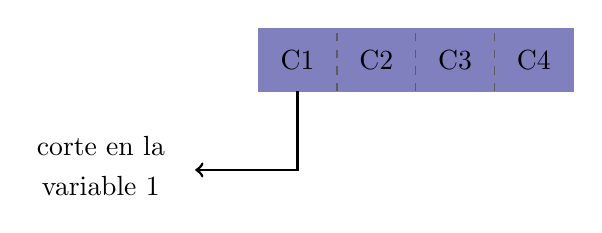
\begin{tikzpicture}[scale=1]
    \colorlet{c1}{blue!50!black!50}
    \colorlet{c2}{red!50!black!50}
    \colorlet{gray}{gray!40!black!80}

    \draw[c1, fill] (0,0.2) rectangle (4,1);

    \draw node at (0.5, 0.6) {C1};
    \draw node at (1.5, 0.6) {C2};
    \draw node at (2.5, 0.6) {C3};
    \draw node at (3.5, 0.6) {C4};

    \foreach \x in {1,2,3} \draw[dashed,gray] (\x,0.2) -- (\x,1);

    %% \draw[->,line width=2] (2,-0.5) -- (2,-2.3);

    %% \draw node at (2, -3) {\small "VAR1$>$C1 \&\& VAR2$>$C2 \&\& VAR3$>$C3 \&\& VAR4$<$C4"};

    \draw node at (-2,-0.5) {corte en la};
    \draw node at (-2,-1) {variable 1};

    \draw[->,line width=1] (0.5,0.2) |- (-0.8,-0.8);

\end{tikzpicture}

  \end{center}

\end{frame}


\begin{frame}[fragile]{Implementaci\'on: Fitness}

  \begin{itemize}\itemsep0.2cm
  \item El \emph{fitness} de un individuo va a ser la significancia de la se\~nal dado el conjunto de cortes representado por el individuo.
  \end{itemize}

  %% 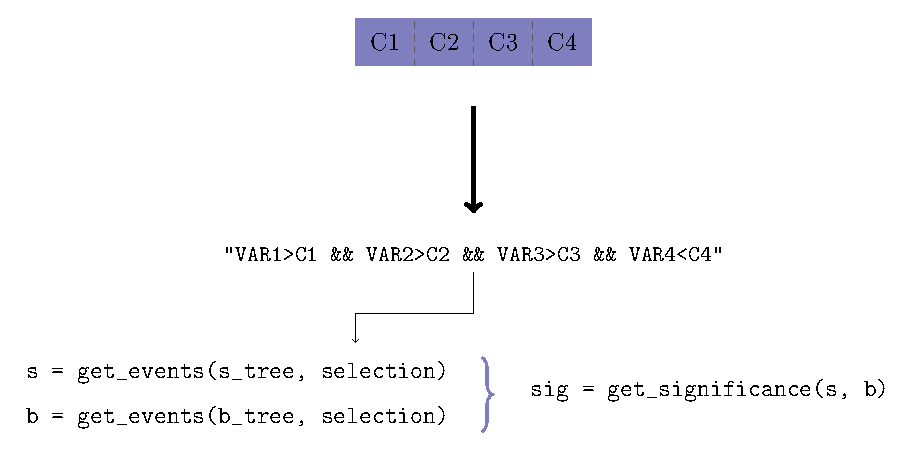
\includegraphics[width=0.6\textwidth]{fitness}
  \scalebox{0.6}{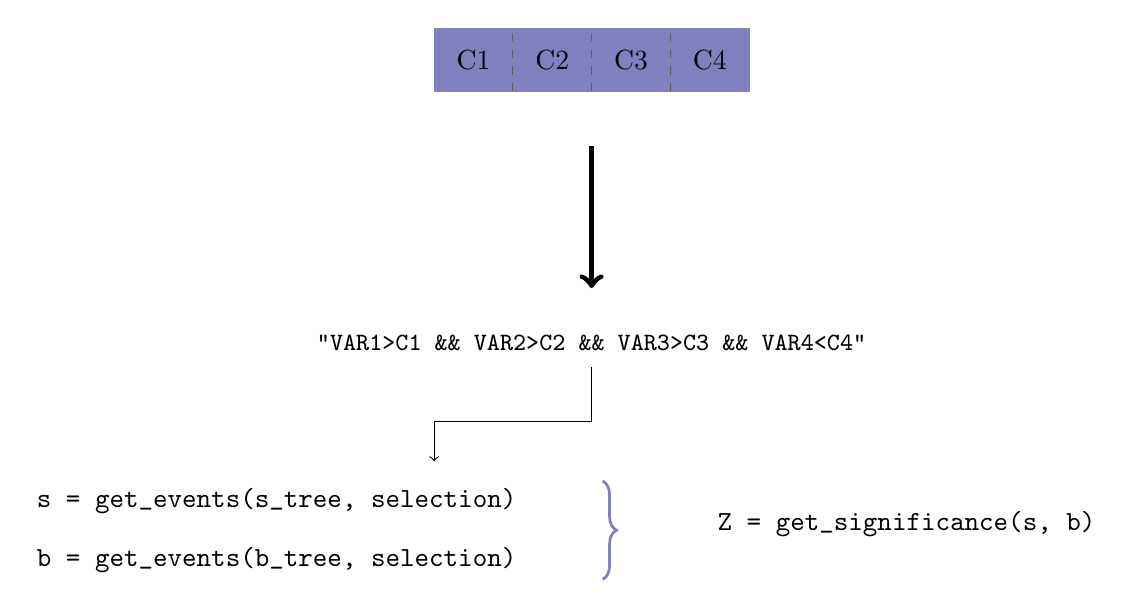
\begin{tikzpicture}
    \colorlet{c1}{blue!50!black!50}
    \colorlet{c2}{red!50!black!50}
    \colorlet{gray}{gray!40!black!80}

    \draw[c1, fill] (0,0.2) rectangle (4,1);

    \draw node at (0.5, 0.6) {C1};
    \draw node at (1.5, 0.6) {C2};
    \draw node at (2.5, 0.6) {C3};
    \draw node at (3.5, 0.6) {C4};

    \foreach \x in {1,2,3} \draw[dashed,gray] (\x,0.2) -- (\x,1);

    \draw[->,line width=2] (2,-0.5) -- (2,-2.3);

    \draw node at (2, -3) {\small \verb|"VAR1>C1 && VAR2>C2 && VAR3>C3 && VAR4<C4"|};

    \draw node at (-2,-5) {\verb|s = get_events(s_tree, selection)|};
    \draw node at (-2,-5.75) {\verb|b = get_events(b_tree, selection)|};

    \draw node at (6, -5.3) {\verb|Z = get_significance(s, b)|};

    \draw [decorate,decoration={brace,amplitude=5pt,mirror,raise=4pt},yshift=0pt,c1,line width=1]
(2,-6) -- (2,-4.75);

    \draw[->] (2,-3.3) |- (0,-4) -| (0,-4.5);

\end{tikzpicture}
}

  \begin{flushleft}
    donde:
  \end{flushleft}

  \begin{itemize}\itemsep0.2cm
  \item \verb|s_tree|, \verb|b_tree| son \verb|TChain| de se\~nal/fondo respectivamente
  \item \texttt{s} y \texttt{b} es el n\'umero de eventos de se\~nal y fondo
  \item \texttt{Z} es la significancia calculada a partir de \texttt{s} y \texttt{b}, que va a ser el fitness del individuo.
  \end{itemize}

\end{frame}

%%\begin{enumerate}
%%   \item Leer archivo de configurari\'on
%%   %%\item
%%   \end{enumerate}


\begin{frame}[fragile]{C\'odigo}

  \begin{flushleft}
    Estructura del c\'odigo
  \end{flushleft}

    \begin{itemize}\itemsep0.6cm
    \item \texttt{main.cpp}
    \item \texttt{ga.cpp, ga.h}
      \oneitem{Implementaci\'on del algoritmo g\'enetico. Todos los par\'ametros son leidos de un archivo de configuraci\'on.}
    \item \texttt{individual.cpp, individual.h}
      \oneitem{Implementaci\'on de la clase individuo.}
    \item \texttt{random.cpp, random.h}
      \oneitem{Funciones \'utiles para generar numeros aleatorios (usando MT)}
    \item \texttt{significance.cpp, significance.h}
      \oneitem{Funciones para calcular significancia.}
    \end{itemize}

    \vspace{0.2cm}

    \begin{flushleft}
      En las siguientes slides se explican las partes principales del c\'odigo.
    \end{flushleft}

\end{frame}

\begin{frame}[fragile]{Funciones random (\texttt{random.cpp})}

  \begin{lstlisting}[language=c++]
#include <random> // random generators
typedef std::mt19937 generator_t;

// init random generator with seed from the system clock
void init_random()
{
  unsigned seed = std::chrono::system_clock::now().time_since_epoch().count();
  generator.seed(seed);
}

// get random integer between lower and upper
int get_random_int(int lower, int upper)
{
  std::uniform_int_distribution<int> distribution(lower, upper);
  return distribution(generator);
}

// get random float between lower and upper
float get_random_float(float lower, float upper)
{
  std::uniform_real_distribution<double> distribution(lower, upper);
  return distribution(generator);
}

// get random probability: float between 0 and 1
float get_random_prob()
{
  return get_random_float(0.0, 1.0);
}
  \end{lstlisting}

\end{frame}

\begin{frame}[fragile]{C\'alculo de significancia (\texttt{significance.cpp}) }

  \begin{lstlisting}[language=c++]
#include <TMath.h>

double get_significance(double s, double b)
{
  if (s < 0 || b < 1)
    return 0.00;

  double sig_2 =  2 * ( (s + b) * TMath::Log(1 + s/b) - s );

  if (sig_2 < 0.00 || std::isinf(sig_2))
    return 0.00;

  return TMath::Sqrt(sig_2);
}
  \end{lstlisting}

\end{frame}

\begin{frame}[fragile]{Clase Individuo (\texttt{individual.h})}

  \begin{lstlisting}[language=c++]
class Individual {

 public:
  Individual();
  ~Individual() {};

  void add_cut(double v) { m_cuts.push_back(v); }
  void set_cut(int idx, double v) { m_cuts[idx] = v; }

  double get_cut(int idx) { return m_cuts[idx]; }
  double* get_cuts();

  void set_fitness(double f) { m_fitness = f; };
  double get_fitness() { return m_fitness; };

  Individual* copy();

 private:
  std::vector<double> m_cuts;
  double m_fitness;
};
  \end{lstlisting}

\end{frame}

\begin{frame}[fragile]{\texttt{ga.cpp}}

  \begin{lstlisting}[language=c++]
    GA::GA(std::string configfile)
{
  read_configuration(configfile);

  init_random();

  // output file
  output.open(m_name+".log");

  // chains
  m_signal_chain = new TChain(m_signal_treename);
  m_signal_chain->AddFile(m_signal_file);

  m_background_chain = new TChain(m_background_treename);
  m_background_chain->AddFile(m_background_file);


  // histograms
  Int_t bins[m_nvars];
  Double_t xmin[m_nvars];
  Double_t xmax[m_nvars];

  for (unsigned int i=0; i<m_nvars; i++) {
    bins[i] = (m_variables[i].max - m_variables[i].min)/m_variables[i].step;
    xmin[i] = m_variables[i].min;
    xmax[i] = m_variables[i].max;
  }

  hist_s   = new THnSparseD("hist_s", "Signal", m_nvars, bins, xmin, xmax);
  hist_b   = new THnSparseD("hist_b", "Background", m_nvars, bins, xmin, xmax);
  hist_sig = new THnSparseD("hist_sig", "Significance", m_nvars, bins, xmin, xmax);

}
\end{lstlisting}

\end{frame}



\begin{frame}[fragile]{\texttt{ga.cpp}: Configuraci\'on}

  \begin{lstlisting}[language=c++]
    void GA::read_configuration(TString configfile)
{
  TEnv env(configfile.Data());

  m_name = env.GetValue("AnalysisName", "output");

  // GA parameters
  m_population_size = env.GetValue("GA.PopulationSize", 0);
  m_generation_max  = env.GetValue("GA.GenerationMax", 10);
  m_prob_mutation   = env.GetValue("GA.ProbMutation", 0.0);
  m_prob_crossover  = env.GetValue("GA.ProbCrossOver", 0.0);
  m_elitism_rate    = env.GetValue("GA.RateElitism", 0.0);

  // Signal
  m_signal_file = env.GetValue("Signal.File", "");
  m_signal_treename = env.GetValue("Signal.TreeName", "");

  // Background
  m_background_file = env.GetValue("Background.File", "");
  m_background_treename = env.GetValue("Background.TreeName", "");
  m_background_syst = env.GetValue("Background.Syst", -1.0);

  // Variables
  m_nvars = env.GetValue("Variable.N", 0);
  m_weight = env.GetValue("Variable.Weight", "");
  m_basesel = env.GetValue("Variable.BaseSelection", "");

  for (unsigned int i=0; i<m_nvars; i++) {
    TString tmp = Form("Variable%i", i+1);

    Variable var;
    var.name = env.GetValue(tmp+".Name", "");
    var.type = env.GetValue(tmp+".Type", ">");
    var.min  = env.GetValue(tmp+".Min", 0.0);
    var.max  = env.GetValue(tmp+".Max", 0.0);
    var.step = env.GetValue(tmp+".Step", 0.0);
    var.bins = int((var.max-var.min)/var.step);

    m_variables.push_back(var);
  }

}
\end{lstlisting}

\end{frame}


\begin{frame}[fragile]{\texttt{ga.cpp}: Un paso del algoritmo gen\'etico}

  \begin{lstlisting}[language=c++]
void GA::step()
{
  pop_vector children;
  children.clear();
  children.reserve(m_population_size);

  // elitism
  unsigned int elite_size = m_population_size * m_elitism_rate;

  for (unsigned int i=0; i<elite_size; i++) {
    children.push_back(m_population[i]->copy());
  }

  // crossover
  while (children.size() < (m_population_size - elite_size)) {

    // select parents
    int p1 = roulette();
    int p2 = roulette();

    // crossover parents
    crossover(m_population[p1], m_population[p2], children);
  }

  // mutation
  mutate(children);

  // update population
  update(children);
  m_generation++;

  // evaluate fitness and sort
  evaluate_fitness();

  // 7. log, save generation
  log();
}
\end{lstlisting}
\end{frame}

\begin{frame}[fragile]{\texttt{main.cpp}}

  \begin{lstlisting}[language=c++]
#include <iostream>

#include "ga.h"

int main(int argc, char *argv[])
{

  if (argc < 2) {
    std::cout << "usage: evolve [CONFIG]" << std::endl;
    return 1;
  }

  GA ga(argv[1]);
  ga.evolve();

  return 0;
}
  \end{lstlisting}
\end{frame}

\begin{frame}[fragile]{Ejemplo}

  \begin{itemize}
  \item Usando los datos de se\~nal y fondo del archivo \texttt{example/data.root} que contienen datos simulados con MC.
  \item Las distribuciones de algunas variables antes de la optimizaci\'on.
  \end{itemize}

  \includegraphics[width=0.40\textwidth]{ph_pt}
  \includegraphics[width=0.40\textwidth]{met_et}

  \includegraphics[width=0.40\textwidth]{jet_n}
  \includegraphics[width=0.40\textwidth]{ht}

\end{frame}


\begin{frame}[fragile]{Ejemplo: Configuraci\'on (\texttt{example/example.conf})}

  \tiny
  \begin{lstlisting}[language=python]
# Configuration Example

AnalysisName: AnalysisExample

# GA options
GA.PopulationSize: 100
GA.GenerationMax: 100
GA.ProbMutation: 0.10
GA.ProbCrossover: 0.90
GA.RateElitism: 0.10

# Signal & Background
Signal.File: example.root
Signal.TreeName: signal
Background.File: example.root
Background.TreeName: background
Background.SystUnc: 0.25

# Variables
Variable.N: 2
Variable.Weight: weight
Variable.BaseSelection: ph_n==1 && el_n==0 && mu_n==0

Variable1.Name: ph_pt
Variable1.Type: >
Variable1.Min: 125.0
Variable1.Max: 500.0
Variable1.Step: 5.0

Variable2.Name: met_et
Variable2.Type: >
Variable2.Min: 100.0
Variable2.Max: 1000.0
Variable2.Step: 10.0
  \end{lstlisting}

\end{frame}

\begin{frame}{Ejemplo: Resultados}

  \begin{itemize}\itemsep0.2cm\parskip0.2cm
  \item Utilizando una poblaci\'on de 100 individuos y 100 generaciones, se alcanza una significancia de
    $\sim 31.7$ para los siguientes calores:

    \begin{itemize}
    \item \texttt{ph\_pt} $> 145$
    \item \texttt{met\_et} $> 300$
    \item \texttt{jet\_n} $>= 4$
    \item \texttt{ht} $> 560$
    \item \texttt{rt2} $< 0.85$
    \end{itemize}

  \end{itemize}

  \includegraphics[width=0.5\textwidth]{sig_vs_generation.pdf}

\end{frame}

\begin{frame}{Conclusi\'on}

  \begin{itemize}\itemsep0.2cm\parskip0.2cm
  \item Se implement\'o un programa para optimizar una selecci\'on de b\'usqueda de nueva f\'isica
    utilizando un algoritmo genetico.
  \item Para esto se utiliz\'o \texttt{C++} y las librerias de \texttt{ROOT}.
  \item Se utiliz\'o el programa a modo de prueba en algunos eventos de se\~nal y fondo simulados
    utilizando generadores de eventos Monte Carlo, dando buenos resultados con un n\'umero
    peque\~no de iteraciones, compatibles con los encontrados utilizando la optimizaci\'on tradicional.

  \item El codigo puede encontrarse en \href{https://github.com/franaln/evolve}{\texttt{https://github.com/franaln/evolve}}

  \end{itemize}


  \end{frame}



\end{document}
